% Intended LaTeX compiler: xelatex
\documentclass[10pt, svgnames]{beamer}
\usepackage{graphicx}
\usepackage{longtable}
\usepackage{wrapfig}
\usepackage{rotating}
\usepackage[normalem]{ulem}
\usepackage{amsmath}
\usepackage{amssymb}
\usepackage{capt-of}
\usepackage{hyperref}
\usetheme{metropolis}
\author{Sappinandana Akamphon}
\date{\today}
\title{Design of Simple Machine Elements}
\subtitle{ME 310: Mechanical Design}
\usepackage{booktabs}
\usepackage{pgfplots}
\usepackage{multirow}
\usepackage{smartdiagram}
\pgfplotsset{compat=1.18}
\definecolor{lightblue}{RGB}{180,220,255}
\institute{Department of Mechanical Engineering, TSE}
\date{}
\usetikzlibrary{patterns,shapes,arrows}
\AtBeginSection[]{\begin{frame}{Outline}\tableofcontents[currentsection]\end{frame}}
\hypersetup{
 pdfauthor={Sappinandana Akamphon},
 pdftitle={Design of Simple Machine Elements},
 pdfkeywords={},
 pdfsubject={},
 pdfcreator={Emacs 30.0.50 (Org mode 9.6)}, 
 pdflang={English}}
\begin{document}

\maketitle

\section{Simple Machine Elements}
\label{sec:org8792df8}

\begin{frame}[label={sec:orge8616ee}]{Not-so-simple Machine Elements}
\begin{itemize}
\item Most elements have multiple loads at once
\item What do we do?
\item Relax. That's what we are here to find out.
\end{itemize}
\end{frame}

\section{Beam Design}
\label{sec:orge45c08c}

\begin{frame}[label={sec:org2a5e1ca}]{Fully Stressed Beams}
\begin{center}
\includegraphics[width=.9\linewidth]{./pictures/fea-beam.png}
\end{center}

\begin{center}
\includegraphics[width=.9\linewidth]{./pictures/fea-fully-stressed-beam.png}
\end{center}
\end{frame}

\begin{frame}[label={sec:org4fe7395}]{Fully Stressed Cantilever Beam}
\begin{center}
\includegraphics[width=.9\linewidth]{./pictures/fea-fully-stressed-beam-analysis.png}
\end{center}

\begin{equation*}
  \sigma(x) = \frac{My}{I} = \frac{Fx(h/2)}{bh^3/12} = \frac{6Fx}{bh^2}
\end{equation*}
\end{frame}

\begin{frame}[label={sec:org8021b01}]{Shape of Fully Stressed Cantilever Beam}
Let \(\sigma(x) = S_y\) for all \(x\)
\begin{gather*}
  \frac{6Fx}{bh^2} = S_y \\
  bh^2 = \frac{6Fx}{S_y} = cx
\end{gather*}
\end{frame}

\begin{frame}[label={sec:orgeef5237}]{Shape of Fully Stressed Cantilever Beam}
\begin{itemize}
\item Set \(b\) as a constant = constant width
\end{itemize}

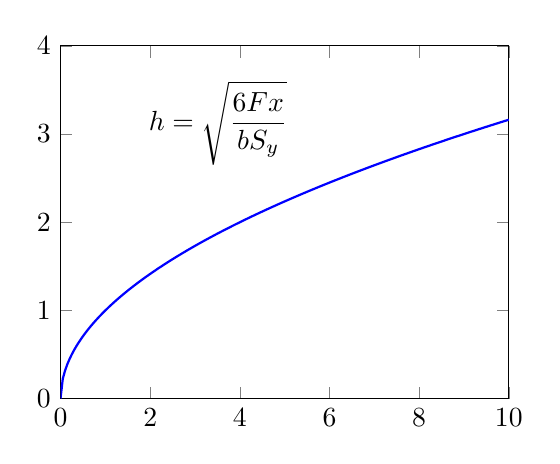
\begin{tikzpicture}
  \begin{axis} [
    height=0.5\textwidth,
    width=0.6\textwidth,
    xmin=0,xmax=10,
    ymin=0,ymax=4,
    ]
    \addplot [domain=0:10,samples=200,no marks, blue, thick] {sqrt(x)};
  \end{axis}
  \node at (2,3.5) {$h = \sqrt{\dfrac{6Fx}{bS_y}}$};
\end{tikzpicture}
\includegraphics[width=0.4\textwidth]{pictures/fully-stressed-parabola}
\end{frame}

\begin{frame}[label={sec:orgde5d8a1}]{Shape of Fully Stressed Cantilever Beam}
\begin{itemize}
\item Set \(h\) as a constant = constant thickness
\end{itemize}

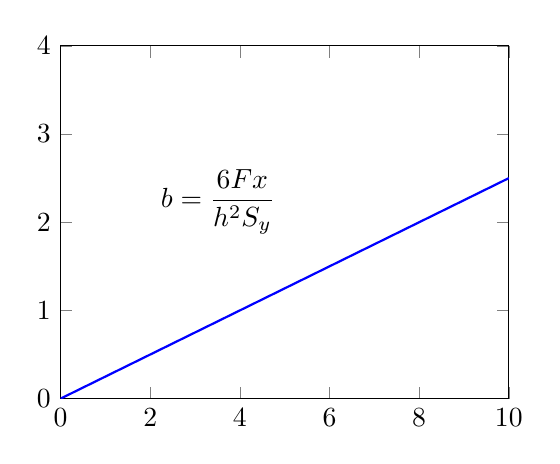
\begin{tikzpicture}
  \begin{axis} [
    height=0.5\textwidth,
    width=0.6\textwidth,
    xmin=0,xmax=10,
    ymin=0,ymax=4,
    ]
    \addplot [domain=0:10,no marks, blue, thick] {x/4};
  \end{axis}
  \node at (2,2.5) {$b = \dfrac{6Fx}{h^2S_y}$};
\end{tikzpicture}
\includegraphics[width=0.4\textwidth]{pictures/fully-stressed-wedge}
\end{frame}

\begin{frame}[label={sec:org3e92343}]{Exercise: Fully Stressed Simply-supported Beams}
\begin{itemize}
\item Find shapes for a simply supported beam with midpoint load
\begin{enumerate}
\item constant \(h\)
\item constant \(b\)
\end{enumerate}
\end{itemize}
\end{frame}

\begin{frame}[label={sec:org93140df}]{Fully Stressed Beam in 3D}
\centering
\includegraphics[width=0.45\textwidth]{pictures/fea-fully-stressed-beam-3d}
\includegraphics[width=0.45\textwidth]{pictures/fea-fully-stressed-beam-3d-section}
\end{frame}


\begin{frame}[label={sec:orgcf22e8e}]{Structural sections of beams}
\begin{figure}
  \centering
  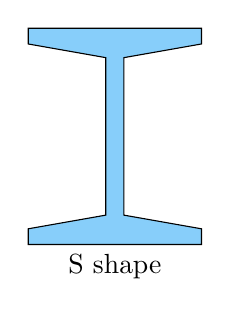
\begin{tikzpicture}
    \draw [fill=LightSkyBlue] (0,0) ++ (0:0.2) --++ (90:1) --++ (10:1) --++ (90:0.2) --++ (180:2.2) --++ (-90:0.2) --++ (-10:1) --++ (-90:2) --++ (-170:1) --++ (-90:0.2) --++ (0:2.2) node[midway, below]{S shape} --++ (90:0.2) --++ (170:1) --cycle;
  \end{tikzpicture}
  \hspace{1cm}
  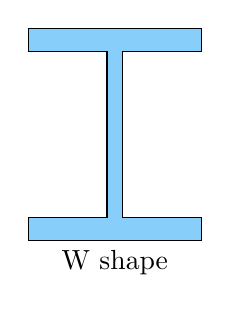
\begin{tikzpicture}
    \draw [fill=LightSkyBlue] (0,0) ++ (0:0.2) --++ (90:1.1) --++ (0:1) --++ (90:0.3) --++ (180:2.2) --++ (-90:0.3) --++ (0:1) --++ (-90:2.1) --++ (180:1) --++ (-90:0.3) --++ (0:2.2) node[midway, below]{W shape} --++ (90:0.3) --++ (180:1) --cycle;
    % \draw [dashed] (0.1,-2) node[below]{2}--++ (90:4) node[above]{2};
    % \draw [dashed] (-1.5,0) node[left]{1} --++ (0:3) node[right]{1};
  \end{tikzpicture}
   \hspace{1cm}
  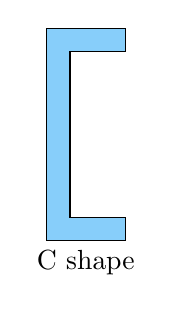
\begin{tikzpicture}
    \draw [fill=LightSkyBlue] (0,0) --++ (180:1) node[midway, below]{C shape} --++ (90:2.7) --++ (0:1) --++ (-90:0.3) --++ (180:0.7) --++ (-90:2.1) --++ (0:0.7) -- cycle;
  \end{tikzpicture}
  \hspace{1cm}
  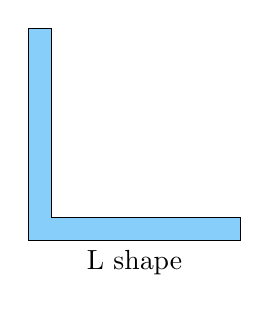
\begin{tikzpicture}
    \draw [fill=LightSkyBlue] (0,0) --++ (0:2.7) node[midway, below]{L shape} --++ (90:0.3) --++ (180:2.4) --++ (90:2.4) --++ (180:0.3) -- cycle;
  \end{tikzpicture}
\end{figure}
\end{frame}

\begin{frame}[label={sec:org7ef1647}]{Beam design constraints}
\begin{itemize}
\item Stress
\item Deformation
\end{itemize}

Which of the conditions is mandatory? Why?
\end{frame}

\begin{frame}[label={sec:org0197609}]{Stress Constraint}
From beam and safety factor equations
\begin{gather*}
  \sigma = \dfrac{My}{I} = \dfrac{M}{S} \\
  N_s = \dfrac{S_y}{\sigma}
\end{gather*}

We have
$$ S = \dfrac{N_s M}{S_y} $$
\end{frame}

\begin{frame}[label={sec:org5944563}]{Deformation Constraint}
\begin{align*}
  \delta &= k \dfrac{FL^3}{EI} \\
  I &= k \dfrac{FL^3}{E \delta}
\end{align*}

\(k\) depends on loading and support conditions
\end{frame}

\begin{frame}[label={sec:org0d4b1dc}]{Example: Gantry Crane}
Select a proper section to build a 3-ton gantry crane of 4-m span. The maximum deflection should be less than 1 cm.

\begin{columns}
\begin{column}{0.6\columnwidth}
\begin{center}
\includegraphics[width=.9\linewidth]{./pictures/gantry-crane.png}
\end{center}
\end{column}
\begin{column}{0.4\columnwidth}
\begin{gather*}
  S_y = 300 \text{ MPa} \\
  \delta = \frac{FL^3}{48EI}
\end{gather*}
\end{column}
\end{columns}
\end{frame}

\begin{frame}[label={sec:org4f3f464}]{Section Properties}
\begin{center}
\includegraphics[width=.9\linewidth]{./pictures/section-table.png}
\end{center}
\end{frame}

\section{Column Design}
\label{sec:org18a313a}
\begin{frame}[label={sec:org51e962d}]{Column constraints}
\begin{itemize}
\item Theoretically we have \(P = \dfrac{\pi^2 EI}{L_e^2}\)
\item Shouldn't that be enough?
\item yielding vs buckling
\end{itemize}
\end{frame}

\begin{frame}[label={sec:org5baf740}]{Real World Columns}
\begin{columns}
\begin{column}{0.4\columnwidth}
\includegraphics[height=0.5\textheight]{pictures/perfect-column} \\\empty
Theory

\begin{itemize}
\item perfectly straight
\item consistent properties
\item centroidal load
\end{itemize}
\end{column}

\begin{column}{0.4\columnwidth}
\includegraphics[height=0.5\textheight]{pictures/real-world-column} \\\empty
Real World

\begin{itemize}
\item not true
\item never true
\item does not happen ever
\end{itemize}
\end{column}
\end{columns}
\end{frame}

\begin{frame}[label={sec:orgc85bc86}]{Column Dimensions and Design Equations}
\begin{itemize}
\item Allowable stress depends on beam \emph{slenderness ratio}
$$ \lambda = \frac{KL}{r_g} $$
\item Need to find a `critical slenderness ratio' \(\lambda_c\) where the same load can cause buckling or yielding
\end{itemize}
\end{frame}


\begin{frame}[label={sec:orgafe2860}]{Steel Column Critical Slenderness Ratio}
\begin{itemize}
\item Critical slenderness ratio \(\lambda_c\) where the same load causes buckling and yielding
\begin{gather*}
  S_y = \frac{\pi ^2E}{\lambda_c^2} \\
  \lambda_c = \sqrt {\frac{\pi^2E}{S_y}}
\end{gather*}
\item longer beams \(\rightarrow\) buckling, shorter beams \(\rightarrow\) yielding
\end{itemize}
\end{frame}

\begin{frame}[label={sec:org5e587d5}]{Column with Eccentric Loads (or Bending Loads)}
\begin{itemize}
\item What if the column is taking a bending load as well?
\item For short columns
\begin{equation*}
  \sigma_{\max} = \frac{P}{A} + \frac{My}{I}
\end{equation*}
\end{itemize}
\end{frame}


\begin{frame}[label={sec:org8b2391c}]{And for longer columns?}
\begin{itemize}
\item Use interaction formula
\begin{gather*}
  A_a = \frac{P}{(\sigma_a)_{allow}} \\
  A_b = \frac{My}{(\sigma _b)_{allow}r_g^2} \\
  A \geqslant A_a + A_b \\
  \dfrac{\sigma _a}{(\sigma_a)_{allow}} + \dfrac{\sigma_b}{(\sigma_b)_{allow}} \leqslant 1
\end{gather*}
\end{itemize}
\end{frame}


\begin{frame}[label={sec:org4449287}]{Example: Column with Bending Load(s)}
Reconsider the gantry crane column example, but now the beam is fixed to the columns. The new safety factor should be 3.
\end{frame}


\begin{frame}[label={sec:org4bf6e67}]{Solution: Column with Bending Loads}
\begin{itemize}
\item Maximum stress happens when the weight is in the middle.
\item The compressive load is that each column takes is \(\dfrac{F}{2}\) = 50000 N.
\item The bending moment caused by midpoint load is \(\dfrac{FL}{8}\) = 50000 N-m
\end{itemize}
\end{frame}

\begin{frame}[label={sec:org635aa04}]{Calculating the ratio}
\begin{itemize}
\item We need to determine the ratio \(\dfrac{\sigma _a}{(\sigma_a)_{allow}} + \dfrac{\sigma_b}{(\sigma_b)_{allow}}\)
\item For steel, \((\sigma_a)_{allow} = (\sigma_b)_{allow} = \sigma_{allow}\)
\item As a sample calculation,
\end{itemize}

\begin{align*}
&\sigma_a = \frac{50000.0}{0.0189} =2645502.6455026455\text{ Pa} \\
&\sigma_b = \frac{50000}{0.00326} = 15337423.312883437\text{ Pa} \\
&\frac{\sigma_a + \sigma_b}{\sigma_{allow}} = 0.18
\end{align*}
\end{frame}

\begin{frame}[label={sec:org04b68fd}]{Solution}
Use data table to generate results

\small
\begin{tabular}{lccc}
\toprule
Designation & Axial Stress & Bending Stress & $\dfrac{\sigma _a + \sigma_b}{\sigma_{allow}}$ \\
\midrule
S610 x 149 & 2.65e+06 & 1.53e+07 & 0.18 \\
S510 x 143 & 2.75e+06 & 1.85e+07 & 0.21 \\
S460 x 104 & 3.79e+06 & 2.96e+07 & 0.33 \\
S380 x 74 & 5.27e+06 & 4.72e+07 & 0.52 \\
S310 x 74 & 5.31e+06 & 6.03e+07 & 0.66 \\
S250 x 52 & 7.52e+06 & 1.04e+08 & 1.11 \\
\bottomrule
\end{tabular}

\normalsize
In this case, S310 x 74 is our pick.
\end{frame}

\section{Shaft Design}
\label{sec:org97b89a6}

\begin{frame}[label={sec:orga42b0e3}]{Shaft Loading Conditions}
\begin{itemize}
\item Torque
\item Bending \(\implies\) radial load from torque transmission
\end{itemize}

\begin{center}
\includegraphics[width=.9\linewidth]{./pictures/torque-transmission.png}
\end{center}

$$ F = \dfrac{T}{r \cos \theta} \hspace{1cm} F = \dfrac{T}{r} \hspace{1cm} F_1 - F_2 = \dfrac{T}{r} $$
\end{frame}

\begin{frame}[label={sec:orgdda63bb}]{Example: Timing Belt Shaft}
Size the shaft (AISI 1040, \(S_y\) = 400 MPa, \(S_{ut}\) = 600 MPa) using

\begin{enumerate}
\item MDET
\item Soderberg theory

\centering
\includegraphics[width=0.7\textwidth]{pictures/shaft-sizing}
\end{enumerate}
\end{frame}

\begin{frame}[label={sec:org2de8864}]{General Guidelines}
\begin{enumerate}
\item shaft should be as short as possible
\item avoid sharp step
\item round shaft if possible
\item to save weight \(\rightarrow\) hollow shaft
\end{enumerate}
\end{frame}

\begin{frame}[label={sec:org5c5564f}]{Typical Shaft Design Equation}
Using stress constraints and MDET

$$ d = \left( \dfrac{4 N_s}{\pi S_y} \sqrt{(8M + Fd)^2 + 48T^2} \right)^{1/3} $$
\end{frame}
\end{document}